% !TEX program = xelatex
% 공통수학2 · Ⅰ. 도형의 방정식 · 02 직선의 위치 관계 · 2/2차시
% 학생용 활동지 (답안 없음)

\documentclass[11pt,a4paper]{article}

\usepackage{kotex}
\usepackage{iftex}
\ifPDFTeX\else
  \setmainhangulfont{Noto Serif CJK KR}
  \setsanshangulfont{Noto Sans CJK KR}
\fi

\usepackage[margin=2.1cm]{geometry}
\usepackage{parskip}
\usepackage{enumitem}
\usepackage{array}
\usepackage{tabularx}
\usepackage{xcolor}
\usepackage{amssymb}
\usepackage{tikz}
\usepackage[most]{tcolorbox}
\usepackage{fancyhdr}
\usepackage{titlesec}

\definecolor{goldc}{HTML}{B07C22}
\definecolor{goldstrong}{HTML}{8A5F16}
\definecolor{indigoc}{HTML}{2B3B57}
\definecolor{indigosoft}{HTML}{6E82A6}
\definecolor{linec}{HTML}{D6DACB}
\definecolor{surface2}{HTML}{E4E8DC}
\definecolor{writeline}{HTML}{C7CCBA}
\definecolor{inksoft}{HTML}{52604F}

\titleformat{\section}{\normalfont\sffamily\bfseries\large\color{indigoc}}{\thesection}{0.6em}{}
\titlespacing{\section}{0pt}{14pt}{6pt}

\newtcolorbox{goalbox}{enhanced, breakable, colback=white, colframe=goldc, boxrule=0.5pt, leftrule=3pt, arc=2pt, left=10pt, right=10pt, top=8pt, bottom=8pt}
\newtcolorbox{sheetbox}{enhanced, breakable, colback=white, colframe=linec, boxrule=0.6pt, arc=3pt, left=11pt, right=11pt, top=9pt, bottom=9pt}

\newcommand{\writespace}[1]{%
  \par\nobreak\vspace{3pt}
  \foreach \n in {1,...,#1} {%
    \noindent\textcolor{writeline}{\rule{\linewidth}{0.4pt}}\par\vspace{0.62cm}%
  }
}
\newcommand{\fillblank}[1]{\makebox[#1]{\hrulefill}}

\pagestyle{fancy}
\fancyhf{}
\renewcommand{\headrulewidth}{0pt}
\fancyfoot[L]{\footnotesize\color{inksoft} 공통수학2 · 2026학년도 2학기 · 지평선고등학교}
\fancyfoot[R]{\footnotesize\color{inksoft} 다음 시간 --- 03 점과 직선 사이의 거리(1)}

\begin{document}

\noindent
\begin{minipage}[b]{0.62\linewidth}
  {\sffamily\footnotesize\color{indigosoft} 공통수학2 · Ⅰ. 도형의 방정식}\\[2pt]
  {\sffamily\bfseries\Large 02 직선의 위치 관계 \textperiodcentered\ 5차시}
\end{minipage}\hfill
\begin{minipage}[b]{0.36\linewidth}
  \raggedleft\small\color{inksoft}
  반\ \fillblank{1.6cm} \quad 번호\ \fillblank{1.6cm}\\[4pt]
  이름\ \fillblank{3.6cm}
\end{minipage}

\vspace{4pt}
\noindent{\color{goldc}\rule{\linewidth}{2.2pt}}
\vspace{10pt}

\begin{goalbox}
\textbf{오늘의 목표}\\
두 직선이 수직이기 위한 조건을 알고, 수직인 직선의 방정식과 선분의 수직이등분선을 구할 수 있다.
\vspace{4pt}

\small\color{inksoft}
$\square$ 자신 있음 \quad $\square$ 조금 헷갈림 \quad $\square$ 처음 봄 \hfill (수업 전 나의 상태에 표시)
\end{goalbox}

\section{생각 열기 --- 직각을 품은 삼각형}

\begin{sheetbox}
좌표평면 위에 세 점 O$(0,0)$, A$(1,3)$, B$(3,-1)$이 있다.

\begin{center}
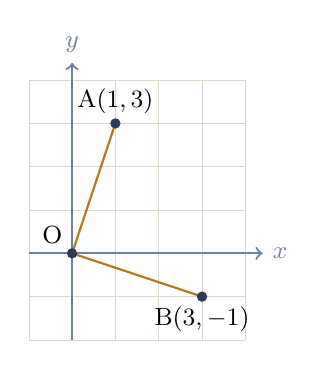
\begin{tikzpicture}[scale=0.55]
  \draw[step=1cm, linec, very thin] (-1,-2) grid (4,4);
  \draw[->, thick, indigosoft] (-1,0) -- (4.4,0) node[right, font=\small]{$x$};
  \draw[->, thick, indigosoft] (0,-2) -- (0,4.4) node[above, font=\small]{$y$};
  \draw[thick, goldc] (0,0) -- (1,3);
  \draw[thick, goldc] (0,0) -- (3,-1);
  \filldraw[indigoc] (0,0) circle (3pt);
  \node[above left, font=\small] at (0,0) {O};
  \filldraw[indigoc] (1,3) circle (3pt);
  \node[above, font=\small] at (1,3) {A$(1,3)$};
  \filldraw[indigoc] (3,-1) circle (3pt);
  \node[below, font=\small] at (3,-1) {B$(3,-1)$};
\end{tikzpicture}
\end{center}

\begin{enumerate}[leftmargin=1.4em, itemsep=2pt]
  \item 세 변 OA, OB, AB의 길이를 각각 구하고, 삼각형 AOB가 직각삼각형인지 확인해 보자.
  \item 직선 OA와 직선 OB의 기울기를 각각 구하고, 두 기울기의 곱을 구해 보자.
\end{enumerate}
\writespace{4}
\end{sheetbox}

\section{개념 정리 --- 두 직선의 수직 조건}

\begin{sheetbox}
두 직선 $y=mx+n$과 $y=m'x+n'$에 대하여

\begin{enumerate}[leftmargin=1.6em, itemsep=4pt]
  \item 두 직선이 서로 수직이면, $mm'=\fillblank{2cm}$
  \item $mm'=-1$이면, 두 직선은 서로 \fillblank{3.6cm}
\end{enumerate}

\vspace{4pt}
\textbf{생각해보기} --- 원점을 지나는 두 직선 $y=mx$, $y=m'x$가 직선 $x=1$과 만나는 점을 각각 P$(1,m)$, Q$(1,m')$이라 하면, 삼각형 POQ가 직각삼각형일 때 피타고라스 정리에 의해
\[
\overline{OP}^2 + \overline{OQ}^2 = \overline{PQ}^2
\]
이 식에 $\overline{OP}^2=1+m^2$, $\overline{OQ}^2=1+m'^2$, $\overline{PQ}^2=(m-m')^2$을 대입하여 정리하면 $mm'=\fillblank{2cm}$을 얻는다.
\end{sheetbox}

\section{연습 문제}

\begin{sheetbox}
\textbf{1.} 점 $(4,1)$을 지나고 직선 $x-2y+2=0$에 수직인 직선의 방정식을 구하시오.
\writespace{2}

\vspace{8pt}
\textbf{2.} 점 $(-2,2)$를 지나고 다음 직선에 수직인 직선의 방정식을 구하시오.\\
\hspace*{1.6em}⑴ $y=2x+5$ \qquad ⑵ $2x+3y-4=0$
\writespace{3}

\vspace{8pt}
\textbf{3. 활동} --- 두 점 A$(-2,-3)$, B$(6,5)$를 이은 선분 AB의 수직이등분선의 방정식을 아래 두 가지 방법으로 각각 구하고, 결과를 비교해 보자.\\[4pt]
\hspace*{1.6em}\textit{방법 1} --- 선분 AB의 중점을 지나고, 직선 AB에 수직인 직선임을 이용.\\[4pt]
\hspace*{1.6em}\textit{방법 2} --- 수직이등분선 위의 점에서 두 점 A, B까지의 거리가 같음을 이용.
\writespace{5}
\end{sheetbox}

\section{사고의 가시화 --- Connect · Extend · Challenge}

\noindent{\footnotesize\color{inksoft} 4차시(평행 조건)와 오늘(수직 조건)을 비교하며 아래 세 칸을 채워 보자.}\\[6pt]
\begin{tabularx}{\linewidth}{@{}XXX@{}}
\textbf{\footnotesize\color{indigoc} Connect --- 평행 조건과 어떻게 연결되나?} &
\textbf{\footnotesize\color{indigoc} Extend --- 새롭게 확장된 것은?} &
\textbf{\footnotesize\color{indigoc} Challenge --- 아직 헷갈리는 것은?} \\[4pt]
\end{tabularx}
\noindent
\begin{minipage}[t]{0.32\linewidth}\writespace{3}\end{minipage}\hfill
\begin{minipage}[t]{0.32\linewidth}\writespace{3}\end{minipage}\hfill
\begin{minipage}[t]{0.32\linewidth}\writespace{3}\end{minipage}

\section{마무리 성찰}

\begin{sheetbox}
\begin{minipage}[t]{0.48\linewidth}
{\footnotesize\color{inksoft} `직선의 위치 관계' 소단원을 마치며 한 문장으로}
\writespace{2}
\end{minipage}\hfill
\begin{minipage}[t]{0.48\linewidth}
{\footnotesize\color{inksoft} 감사 일기 / 유념 한 줄}
\writespace{2}
\end{minipage}
\end{sheetbox}

\end{document}
